% Generated by Sphinx.
\def\sphinxdocclass{article}
\documentclass[letterpaper,10pt,english]{sphinxhowto}
\usepackage[utf8]{inputenc}
\DeclareUnicodeCharacter{00A0}{\nobreakspace}
\usepackage[T1]{fontenc}
\usepackage{babel}
\usepackage{times}
\usepackage[Bjarne]{fncychap}
\usepackage{longtable}
\usepackage{sphinx}
\usepackage{multirow}

\setcounter{page}{1}
\pagenumbering{arabic}


\title{MASS Software Manual}
\date{August 25, 2014}
\release{v1.1}
\author{Jimit Doshi}
\newcommand{\sphinxlogo}{}
\renewcommand{\releasename}{Release}
\makeindex

\makeatletter
\def\PYG@reset{\let\PYG@it=\relax \let\PYG@bf=\relax%
    \let\PYG@ul=\relax \let\PYG@tc=\relax%
    \let\PYG@bc=\relax \let\PYG@ff=\relax}
\def\PYG@tok#1{\csname PYG@tok@#1\endcsname}
\def\PYG@toks#1+{\ifx\relax#1\empty\else%
    \PYG@tok{#1}\expandafter\PYG@toks\fi}
\def\PYG@do#1{\PYG@bc{\PYG@tc{\PYG@ul{%
    \PYG@it{\PYG@bf{\PYG@ff{#1}}}}}}}
\def\PYG#1#2{\PYG@reset\PYG@toks#1+\relax+\PYG@do{#2}}

\expandafter\def\csname PYG@tok@gd\endcsname{\def\PYG@tc##1{\textcolor[rgb]{0.63,0.00,0.00}{##1}}}
\expandafter\def\csname PYG@tok@gu\endcsname{\let\PYG@bf=\textbf\def\PYG@tc##1{\textcolor[rgb]{0.50,0.00,0.50}{##1}}}
\expandafter\def\csname PYG@tok@gt\endcsname{\def\PYG@tc##1{\textcolor[rgb]{0.00,0.27,0.87}{##1}}}
\expandafter\def\csname PYG@tok@gs\endcsname{\let\PYG@bf=\textbf}
\expandafter\def\csname PYG@tok@gr\endcsname{\def\PYG@tc##1{\textcolor[rgb]{1.00,0.00,0.00}{##1}}}
\expandafter\def\csname PYG@tok@cm\endcsname{\let\PYG@it=\textit\def\PYG@tc##1{\textcolor[rgb]{0.25,0.50,0.56}{##1}}}
\expandafter\def\csname PYG@tok@vg\endcsname{\def\PYG@tc##1{\textcolor[rgb]{0.73,0.38,0.84}{##1}}}
\expandafter\def\csname PYG@tok@m\endcsname{\def\PYG@tc##1{\textcolor[rgb]{0.13,0.50,0.31}{##1}}}
\expandafter\def\csname PYG@tok@mh\endcsname{\def\PYG@tc##1{\textcolor[rgb]{0.13,0.50,0.31}{##1}}}
\expandafter\def\csname PYG@tok@cs\endcsname{\def\PYG@tc##1{\textcolor[rgb]{0.25,0.50,0.56}{##1}}\def\PYG@bc##1{\setlength{\fboxsep}{0pt}\colorbox[rgb]{1.00,0.94,0.94}{\strut ##1}}}
\expandafter\def\csname PYG@tok@ge\endcsname{\let\PYG@it=\textit}
\expandafter\def\csname PYG@tok@vc\endcsname{\def\PYG@tc##1{\textcolor[rgb]{0.73,0.38,0.84}{##1}}}
\expandafter\def\csname PYG@tok@il\endcsname{\def\PYG@tc##1{\textcolor[rgb]{0.13,0.50,0.31}{##1}}}
\expandafter\def\csname PYG@tok@go\endcsname{\def\PYG@tc##1{\textcolor[rgb]{0.20,0.20,0.20}{##1}}}
\expandafter\def\csname PYG@tok@cp\endcsname{\def\PYG@tc##1{\textcolor[rgb]{0.00,0.44,0.13}{##1}}}
\expandafter\def\csname PYG@tok@gi\endcsname{\def\PYG@tc##1{\textcolor[rgb]{0.00,0.63,0.00}{##1}}}
\expandafter\def\csname PYG@tok@gh\endcsname{\let\PYG@bf=\textbf\def\PYG@tc##1{\textcolor[rgb]{0.00,0.00,0.50}{##1}}}
\expandafter\def\csname PYG@tok@ni\endcsname{\let\PYG@bf=\textbf\def\PYG@tc##1{\textcolor[rgb]{0.84,0.33,0.22}{##1}}}
\expandafter\def\csname PYG@tok@nl\endcsname{\let\PYG@bf=\textbf\def\PYG@tc##1{\textcolor[rgb]{0.00,0.13,0.44}{##1}}}
\expandafter\def\csname PYG@tok@nn\endcsname{\let\PYG@bf=\textbf\def\PYG@tc##1{\textcolor[rgb]{0.05,0.52,0.71}{##1}}}
\expandafter\def\csname PYG@tok@no\endcsname{\def\PYG@tc##1{\textcolor[rgb]{0.38,0.68,0.84}{##1}}}
\expandafter\def\csname PYG@tok@na\endcsname{\def\PYG@tc##1{\textcolor[rgb]{0.25,0.44,0.63}{##1}}}
\expandafter\def\csname PYG@tok@nb\endcsname{\def\PYG@tc##1{\textcolor[rgb]{0.00,0.44,0.13}{##1}}}
\expandafter\def\csname PYG@tok@nc\endcsname{\let\PYG@bf=\textbf\def\PYG@tc##1{\textcolor[rgb]{0.05,0.52,0.71}{##1}}}
\expandafter\def\csname PYG@tok@nd\endcsname{\let\PYG@bf=\textbf\def\PYG@tc##1{\textcolor[rgb]{0.33,0.33,0.33}{##1}}}
\expandafter\def\csname PYG@tok@ne\endcsname{\def\PYG@tc##1{\textcolor[rgb]{0.00,0.44,0.13}{##1}}}
\expandafter\def\csname PYG@tok@nf\endcsname{\def\PYG@tc##1{\textcolor[rgb]{0.02,0.16,0.49}{##1}}}
\expandafter\def\csname PYG@tok@si\endcsname{\let\PYG@it=\textit\def\PYG@tc##1{\textcolor[rgb]{0.44,0.63,0.82}{##1}}}
\expandafter\def\csname PYG@tok@s2\endcsname{\def\PYG@tc##1{\textcolor[rgb]{0.25,0.44,0.63}{##1}}}
\expandafter\def\csname PYG@tok@vi\endcsname{\def\PYG@tc##1{\textcolor[rgb]{0.73,0.38,0.84}{##1}}}
\expandafter\def\csname PYG@tok@nt\endcsname{\let\PYG@bf=\textbf\def\PYG@tc##1{\textcolor[rgb]{0.02,0.16,0.45}{##1}}}
\expandafter\def\csname PYG@tok@nv\endcsname{\def\PYG@tc##1{\textcolor[rgb]{0.73,0.38,0.84}{##1}}}
\expandafter\def\csname PYG@tok@s1\endcsname{\def\PYG@tc##1{\textcolor[rgb]{0.25,0.44,0.63}{##1}}}
\expandafter\def\csname PYG@tok@gp\endcsname{\let\PYG@bf=\textbf\def\PYG@tc##1{\textcolor[rgb]{0.78,0.36,0.04}{##1}}}
\expandafter\def\csname PYG@tok@sh\endcsname{\def\PYG@tc##1{\textcolor[rgb]{0.25,0.44,0.63}{##1}}}
\expandafter\def\csname PYG@tok@ow\endcsname{\let\PYG@bf=\textbf\def\PYG@tc##1{\textcolor[rgb]{0.00,0.44,0.13}{##1}}}
\expandafter\def\csname PYG@tok@sx\endcsname{\def\PYG@tc##1{\textcolor[rgb]{0.78,0.36,0.04}{##1}}}
\expandafter\def\csname PYG@tok@bp\endcsname{\def\PYG@tc##1{\textcolor[rgb]{0.00,0.44,0.13}{##1}}}
\expandafter\def\csname PYG@tok@c1\endcsname{\let\PYG@it=\textit\def\PYG@tc##1{\textcolor[rgb]{0.25,0.50,0.56}{##1}}}
\expandafter\def\csname PYG@tok@kc\endcsname{\let\PYG@bf=\textbf\def\PYG@tc##1{\textcolor[rgb]{0.00,0.44,0.13}{##1}}}
\expandafter\def\csname PYG@tok@c\endcsname{\let\PYG@it=\textit\def\PYG@tc##1{\textcolor[rgb]{0.25,0.50,0.56}{##1}}}
\expandafter\def\csname PYG@tok@mf\endcsname{\def\PYG@tc##1{\textcolor[rgb]{0.13,0.50,0.31}{##1}}}
\expandafter\def\csname PYG@tok@err\endcsname{\def\PYG@bc##1{\setlength{\fboxsep}{0pt}\fcolorbox[rgb]{1.00,0.00,0.00}{1,1,1}{\strut ##1}}}
\expandafter\def\csname PYG@tok@kd\endcsname{\let\PYG@bf=\textbf\def\PYG@tc##1{\textcolor[rgb]{0.00,0.44,0.13}{##1}}}
\expandafter\def\csname PYG@tok@ss\endcsname{\def\PYG@tc##1{\textcolor[rgb]{0.32,0.47,0.09}{##1}}}
\expandafter\def\csname PYG@tok@sr\endcsname{\def\PYG@tc##1{\textcolor[rgb]{0.14,0.33,0.53}{##1}}}
\expandafter\def\csname PYG@tok@mo\endcsname{\def\PYG@tc##1{\textcolor[rgb]{0.13,0.50,0.31}{##1}}}
\expandafter\def\csname PYG@tok@mi\endcsname{\def\PYG@tc##1{\textcolor[rgb]{0.13,0.50,0.31}{##1}}}
\expandafter\def\csname PYG@tok@kn\endcsname{\let\PYG@bf=\textbf\def\PYG@tc##1{\textcolor[rgb]{0.00,0.44,0.13}{##1}}}
\expandafter\def\csname PYG@tok@o\endcsname{\def\PYG@tc##1{\textcolor[rgb]{0.40,0.40,0.40}{##1}}}
\expandafter\def\csname PYG@tok@kr\endcsname{\let\PYG@bf=\textbf\def\PYG@tc##1{\textcolor[rgb]{0.00,0.44,0.13}{##1}}}
\expandafter\def\csname PYG@tok@s\endcsname{\def\PYG@tc##1{\textcolor[rgb]{0.25,0.44,0.63}{##1}}}
\expandafter\def\csname PYG@tok@kp\endcsname{\def\PYG@tc##1{\textcolor[rgb]{0.00,0.44,0.13}{##1}}}
\expandafter\def\csname PYG@tok@w\endcsname{\def\PYG@tc##1{\textcolor[rgb]{0.73,0.73,0.73}{##1}}}
\expandafter\def\csname PYG@tok@kt\endcsname{\def\PYG@tc##1{\textcolor[rgb]{0.56,0.13,0.00}{##1}}}
\expandafter\def\csname PYG@tok@sc\endcsname{\def\PYG@tc##1{\textcolor[rgb]{0.25,0.44,0.63}{##1}}}
\expandafter\def\csname PYG@tok@sb\endcsname{\def\PYG@tc##1{\textcolor[rgb]{0.25,0.44,0.63}{##1}}}
\expandafter\def\csname PYG@tok@k\endcsname{\let\PYG@bf=\textbf\def\PYG@tc##1{\textcolor[rgb]{0.00,0.44,0.13}{##1}}}
\expandafter\def\csname PYG@tok@se\endcsname{\let\PYG@bf=\textbf\def\PYG@tc##1{\textcolor[rgb]{0.25,0.44,0.63}{##1}}}
\expandafter\def\csname PYG@tok@sd\endcsname{\let\PYG@it=\textit\def\PYG@tc##1{\textcolor[rgb]{0.25,0.44,0.63}{##1}}}

\def\PYGZbs{\char`\\}
\def\PYGZus{\char`\_}
\def\PYGZob{\char`\{}
\def\PYGZcb{\char`\}}
\def\PYGZca{\char`\^}
\def\PYGZam{\char`\&}
\def\PYGZlt{\char`\<}
\def\PYGZgt{\char`\>}
\def\PYGZsh{\char`\#}
\def\PYGZpc{\char`\%}
\def\PYGZdl{\char`\$}
\def\PYGZhy{\char`\-}
\def\PYGZsq{\char`\'}
\def\PYGZdq{\char`\"}
\def\PYGZti{\char`\~}
% for compatibility with earlier versions
\def\PYGZat{@}
\def\PYGZlb{[}
\def\PYGZrb{]}
\makeatother

\begin{document}

\maketitle
\tableofcontents
\phantomsection\label{index::doc}\pagebreak\pagestyle{headings}


\textbf{Multi Atlas Skull Stripping (MASS)}
{[}\href{http://www.sciencedirect.com/science/article/pii/S1076633213004182}{ARAD2013}{]},
is a software package designed for robust and accurate brain extraction, applicable for both individual as well as large population studies.

MASS is implemented as a Unix command-line tool. It is fully automatic and easy to use --- users input
an image, and MASS will output the extracted brain and the associated brain mask.
\pagebreak

\section{About the Algorithm}
\label{about:overview}\label{about::doc}\label{about:about-the-algorithm}
A general overview of the proposed method is given in the following figure.
The MASS framework consists of 3 components: template selection, registration and
label fusion.
\phantomsection\label{about:fig-framework}\begin{quote}
\begin{figure}[htbp]
\centering

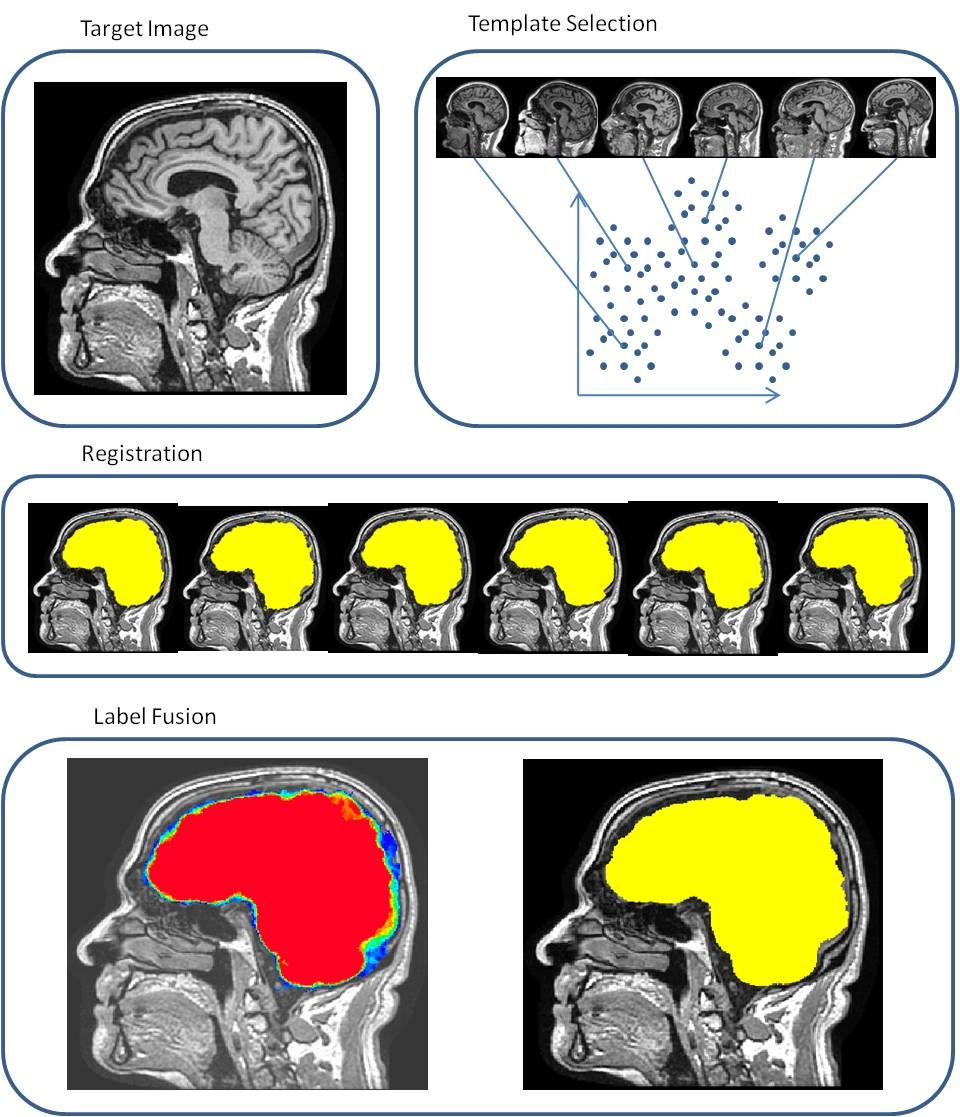
\includegraphics[width=0.900\linewidth]{Figure1_OutlineOfMethod.jpg}
\end{figure}
\end{quote}


\subsection{Template Selection}
\label{about:template-selection}
The quality of a registration is directly related to the similarity between
the template and the target images. Either due to differences between populations
(e.g. age, disease, etc.) or changes in scanner type, technology and
protocol (e.g. 1.5T to 3T), images from two different projects might be significantly
different. In order to increase the template-subject similarity, and
hence to improve the registration accuracy, we select a study-specific set of
templates using a clustering-based approach. The same set of templates is used
for processing all images in the study. In this way, we limit the work required
for the preparation of the ground-truth brain masks, while using templates as similar
as possible to the subjects in the study.


\subsection{Registration}
\label{about:registration}
We have chosen a recently developed publicly available registration method
DRAMMS because of its ability to meet two major challenges specific
to registering raw brain MR images. The first major challenge is the large
amount of intensity inhomogeneity and background noise in raw brain MR
images. DRAMMS finds voxel-wise correspondences by looking at multi-scale
and multi-orientation Gabor texture features around each voxel. Therefore,
it is relatively robust to inhomogeneity and noise. The second major challenge
in registering brain MR images with skull is the possible presence of
outlier regions. Outlier regions, or missing correspondences, usually refer to
regions that exist in one image but not in the other. For instance, the MR
image of one subject may contain more neck regions, or may have part of
superior skull missing due to different field-of-view (FOV) during MRI acquisition.
DRAMMS meets this challenge using the mutual salience weighting,
as it adaptively finds and relies on voxels/regions that are more likely to
establish reliable correspondences across images. This way, it reduces the
negative impact of outlier regions compared to other registration methods
that forces matching for all voxels/regions.


\subsection{Label Fusion}
\label{about:label-fusion}
We adopt a spatially adaptive fusion strategy that takes into consideration
the local similarities between the templates and the target image. At
each voxel, a weight is assigned to each template such that a higher confidence
is given to templates that are locally more similar, e.g. more easily
mapped, to the target image. Our main premise here is that the Jacobian
maps are good indicators of local similarities between source and target images.
Large Jacobian values often correlate with large geometric differences
between template and target images. It’s preferable to assign high weights
to labels from masks that are locally similar to the subject image, as we
have more confidence on the registration when the source and target images
are more similar. Such a weighting mechanism is also efficient for making
the method more robust. If the registration of one (or a few in the extreme
case) template completely fails, the corresponding Jacobian map will have
extreme values in most voxels. Thus the brain mask from this template will
be ranked very low in general, and the template will not have any effect on
the final extraction/segmentation.
\pagebreak

\section{Download}
\label{download:download}\label{download::doc}

\subsection{Software License}
\label{download:software-license}
The MASS software is freely available under a BSD-style open source license that is compatible
with the Open Source Definition by \href{http://opensource.org/}{The Open Source Initiative} and contains no restrictions
on use of the software. The full \href{http://www.cbica.upenn.edu/sbia/software/license.html}{license} text is included with the distribution package and
available online.


\subsection{Documentation}
\label{download:documentation}\label{download:license}
\href{http://www.cbica.upenn.edu/sbia/software/mass/MASS\_Software\_Manual.pdf}{MASS Manual}:
Online version of this manual.


\subsection{System Requirements}
\label{download:system-requirements}
\textbf{Operating System:} Linux


\subsection{Register for Download}
\label{download:register-for-download}\label{download:register}
Please \href{http://www.cbica.upenn.edu/sbia/software/mass/download.html\#register}{\textbf{register online}} to receive an email with the download links of the software.
\pagebreak\pagebreak

\section{Installation}
\label{installation:installation}\label{installation:register-online}\label{installation::doc}
See the \href{http://www.cbica.upenn.edu/sbia/software/basis/howto/install.html}{BASIS guide on software installation} for a complete list of build tools and
detailed installation instructions.


\subsection{Prerequisites}
\label{installation:prerequisites}
\begin{tabulary}{\linewidth}{|p{3.75cm}|m{1.5cm}|p{10cm}|}
\hline
\textbf{
Dependency
} & \textbf{
Version*
} & \textbf{
Description
}\\\hline

\href{http://www.cbica.upenn.edu/sbia/software/basis/index.html}{BASIS}
 & 
2.1.2
 & 
A meta-project developed at \href{http://www.cbica.upenn.edu/sbia/index.html}{SBIA} to standardize the software development.
\\\hline

\href{http://www.cbica.upenn.edu/sbia/software/dramms/download.html}{DRAMMS}
 & 
1.4.1
 & 
A registration algorithm developed at \href{http://www.cbica.upenn.edu/sbia/index.html}{SBIA} to warp images.
\\\hline

\href{http://afni.nimh.nih.gov/afni/download}{AFNI}
 &  & 
Using the version built on 2008\_07\_18\_1710
\\\hline

\href{http://fsl.fmrib.ox.ac.uk/fsl/fslwiki/FslInstallation}{FSL}
 & 
4.1.5
 & 
A comprehensive library of analysis tools for brain imaging data
\\\hline

\href{http://scikit-learn.org/stable/install.html}{SCIKIT-LEARN}
 & 
0.14.1
 & 
A python package providing several data mining and data analysis tools.
\\\hline

\href{http://nipy.org/nibabel/installation.html}{NIBABEL}
 & 
1.2.0
 & 
A python package for read and write access to common medical file formats
\\\hline
\end{tabulary}


* The versions listed are the minimum versions of the softwares for which the MASS package was tested.


\subsection{Job Scheduler}
\label{installation:job-scheduler}
If you have access to a computing cluster which has a job scheduler/queuing software (SGE, PBS etc) installed, it
can be used to significantly reduce the (wall-clock) time it will take for the MASS software to produce the results.
During the installation process, you can initialize the \code{SCHEDULER} variable with the particular version of your
job scheduler. Currently, there are four options that are supported. You can select the one that best fits your system:

\begin{Verbatim}[commandchars=\\\{\}]
SGE  - Sun Grid Engine
PBS  - Portable Batch System
NONE - No queuing system (default)
MISC - User defined setting
\end{Verbatim}

If you have a different queuing software and you select the ``MISC'' option, you need to modify the
\textbf{src/schedulerSettings/SettingsMISC.sh} file within the package with the appropriate options and arguments that are specific
to your queuing system. You can refer to the corresponding files for SGE and PBS as examples.


\subsection{Configure}
\label{installation:configure}\begin{enumerate}
\item {} 
Extract source files:

\begin{Verbatim}[commandchars=\\\{\}]
tar -xzf mass-1.1.0-source.tar.gz
\end{Verbatim}

\item {} 
Create build directory:

\begin{Verbatim}[commandchars=\\\{\}]
mkdir mass-1.1.0-build
\end{Verbatim}

\item {} 
Change to build directory:

\begin{Verbatim}[commandchars=\\\{\}]
cd mass-1.1.0-build
\end{Verbatim}

\item {} 
Run \href{http://www.cmake.org/}{CMake} to configure the build tree by using either one of the following commands:

\begin{Verbatim}[commandchars=\\\{\}]
cmake -D CMAKE\_INSTALL\_PREFIX:STRING=/Full/path/to/install/mass/
      -D SCHEDULER:STRING=??? ../mass-1.1.0-source
\end{Verbatim}

OR:

\begin{Verbatim}[commandchars=\\\{\}]
ccmake ../mass-1.1.0-source
\end{Verbatim}
\begin{itemize}
\item {} 
Press \code{c} to configure the build system and \code{e} to ignore warnings.

\item {} 
Set \code{SCHEDULER} variable with your job scheduler information.

\item {} 
Set \code{CMAKE\_INSTALL\_PREFIX} and other CMake variables and options.

\item {} 
Continue pressing \code{c} until the option \code{g} is available.

\item {} 
Then press \code{g} to generate the \href{http://www.gnu.org/software/make/}{GNU Make} configuration files.

\end{itemize}

\end{enumerate}


\subsection{Build}
\label{installation:build}
After the configuration of the build tree, the software can be built using \href{http://www.gnu.org/software/make/}{GNU Make}:

\begin{Verbatim}[commandchars=\\\{\}]
\PYG{n}{make}
\end{Verbatim}


\subsection{Test}
\label{installation:test}
After building the software, the software tests can be run using

\begin{Verbatim}[commandchars=\\\{\}]
make test
\end{Verbatim}

Allow 30-60 mins for the tests to finish. The last test, if the \code{SCHEDULER} variable is not
set to \code{NONE}, is meant to check if submitting the jobs to the queuing system works. Please
check your queue (for e.g. using \code{qstat} for SGE, PBS) to make sure that the jobs were submitted.
If they are submitted, you can either delete them or wait for them to finish. As soon as these tests
finish, you can proceed to the installation.


\subsection{Install}
\label{installation:install}
The final installation copies the built files and additional data and documentation
files to the installation directory specified using the \code{CMAKE\_INSTALL\_PREFIX}
option during the configuration of the build tree:

\begin{Verbatim}[commandchars=\\\{\}]
make install
\end{Verbatim}

After the successful installation, the build directory can be removed again.
\pagebreak

\section{Manual}
\label{manual::doc}\label{manual:id2}\label{manual:commandlinetools}\label{manual:manual}

\subsection{General Processing Pipeline}
\label{manual:general-processing-pipeline}\begin{description}
\item[{Step 1.}] \leavevmode
Bias correct (N3, N4 or any other method) all of the images so that
any large scale inhomogeneities are removed and the input is of reasonable quality

\item[{Step 2.}] \leavevmode
Run \code{ChooseTemplates} to select a set of subjects (7-20) to be used as templates
for your entire study. If your study is large with a lot of variation (multi site,
multi protocol etc), use more templates.

\item[{Step 3.}] \leavevmode
Run \code{mass} on the bias corrected images selected in \textbf{Step 2} to skullstrip them using
the generic templates provided along with the package. These subjects would be your
gold standard for the rest of your study, so make sure the quality of the results on
these subjects is good. You can manually correct these subjects if you choose to.

\item[{Step 4.}] \leavevmode
Rename these results in the following format, with \emph{N} being the template number from 1 to \emph{N}:

\emph{TemplateN.nii.gz}           - The original intensity image.

\emph{TemplateN\_str\_cbq.nii.gz}   - The brain mask.

\item[{Step 5.}] \leavevmode
Run \code{mass} on all subjects using these new templates by specifying the \code{-ref} option to use
the newly created study-specific templates.

\item[{Step 6.}] \leavevmode
Alternatively, you can skip steps 2-4 and use the generic templates on all of your subjects directly!

\end{description}


\subsection{Template Selection}
\label{manual:template-selection}
The template selection command within MASS which selects the cluster-centers within
the dataset is named \code{ChooseTemplates}. The simplest use is:

\begin{Verbatim}[commandchars=\\\{\}]
\PYG{n}{ChooseTemplates} \PYG{o}{\PYGZhy{}}\PYG{n+nb}{list} \PYG{o}{/}\PYG{n}{path}\PYG{o}{/}\PYG{n}{to}\PYG{o}{/}\PYG{n+nb}{list}\PYG{o}{/}\PYG{n}{of}\PYG{o}{/}\PYG{n}{images}\PYG{o}{.}\PYG{n}{lst}
\end{Verbatim}

This command will return a set of 6 images from the list that are the centroids of
different clusters (k=6). Internally, it first resamples all of the input images to
voxel dimensions 2:2:2 to enhance the processing speed and also reducing the memory
requirement of the process. It then affinely registers all of the input images
to the first image within the input list. So if you have a lot of images within the
list, it may take a some time for it to process those images. In the last step of this
process, it runs the \code{choosetemplates} executable which loads all the affinely
registered images into memory and selects the cluster-centers.

If you have access to the computing cluster, it is \textbf{highly recommended} that you
affinely register (using \code{flirt} with 12 dof) all of the input images to one of the
randomly chosen images yourself and use the \code{-a} option as shown below to notify
the script that the input images are already affinely registered. This will reduce
the processing time significantly.

\textbf{Supported File Formats:} \href{http://nifti.nimh.nih.gov/nifti-1/}{NIfTI-1} (recommended)

\textbf{Supported Datatypes:} byte (unsigned char, uint8), int8, short, int16, uint16, float, float32, int32.

Alternatively, the number of desired clusters can be specified
using the \code{-clust} option as:

\begin{Verbatim}[commandchars=\\\{\}]
ChooseTemplates -list /path/to/list/of/images.lst -clust 15
\end{Verbatim}

If you would like to speed up the processing within this command, you can use multiple
CPU cores on the cluster or on your computer using the \code{-MT} option :

\begin{Verbatim}[commandchars=\\\{\}]
ChooseTemplates -list /path/to/list/of/images.lst -clust 15 -MT 6
\end{Verbatim}

If you have already affinely registered all input images so they are in the same space,
you can specify that by using the \code{-a} option. Here, you do not need the \code{-MT} option
as all images have already been registered :

\begin{Verbatim}[commandchars=\\\{\}]
ChooseTemplates -list /path/to/list/of/images.lst -clust 15 -a
\end{Verbatim}

Additionally, you can also submit this script to your computing cluster if you have a large number
of images that need be clustered. Make sure that you use the appropriate options for requesting memory
as well as the number of threads while submitting this script cluster. This will ensure that the script
does not run out of memory or overload the cluster.


\subsection{MASS Default Command}
\label{manual:mass-default-command}
The main command of MASS which removes the skull and other non-brain tissues
is named \code{mass}. The simplest use is:

\begin{Verbatim}[commandchars=\\\{\}]
mass  -in /path/to/source/sourceimage.hdr
\end{Verbatim}

This command will generate 3 files in the /path/to/source/ directory:
\begin{quote}

\emph{sourceimage\_brain.nii.gz}              - The skull-stripped image

\emph{sourceimage\_brainmask.nii.gz}          - The final brain mask

\emph{sourceimage\_brain\_JacRank.nii.gz}      - The Jacobian Rank Mask
\end{quote}

The Jacobian Rank Mask is a combination of the different registrations weighted locally by their jacobian
determinants. This file can be thresholded using \code{mass-thresholdjacobian} to create stricter or more lenient
masks. The maximum value within this file can vary with the number of templates that are used for registrations.
Since it is a sum of ranks, that max value will always be \code{N*(N+1)/2}, where \code{N} is the number of templates used.

\textbf{Supported File Formats:} \href{http://nifti.nimh.nih.gov/nifti-1/}{NIfTI-1} (recommended)

\textbf{Supported Datatypes:} byte (unsigned char, uint8), int8, short, int16, uint16, float, float32, int32.


\subsection{MASS Options}
\label{manual:id2}\label{manual:mass-options}
To run the mass script which will internally do the processing and then submit the
\code{mass-registrations} and \code{mass-skullStripping} jobs:

\begin{Verbatim}[commandchars=\\\{\}]
mass
 -in /Path/To/Source/Directory/Input\_n3.nii.gz
 -dest /Path/To/Destination/Directory/;
\end{Verbatim}

To use the templates without the cerebellum:

\begin{Verbatim}[commandchars=\\\{\}]
mass
 -in /Path/To/Source/Directory/Input\_n3.nii.gz
 -dest /Path/To/Destination/Directory/
 -noCere;
\end{Verbatim}

To use a user defined set of templates:

\begin{Verbatim}[commandchars=\\\{\}]
mass
 -in /Path/To/Source/Directory/Input\_n3.nii.gz
 -dest /Path/To/Destination/Directory/
 -ref /Path/To/User/Defined/Templates/;
\end{Verbatim}

To remove the skull from the input image using the default options. However, do
not use the computing cluster but run the \code{mass-registrations} jobs serially :

\begin{Verbatim}[commandchars=\\\{\}]
mass
 -in /Path/To/Source/Directory/Input\_n3.nii.gz
 -dest /Path/To/Destination/Directory/
 -NOQ;
\end{Verbatim}

To remove the skull from the input image using the default options, but without
the computing cluster. Additionally, use 6 CPU cores during \code{mass-registrations}
to speed up the process:

\begin{Verbatim}[commandchars=\\\{\}]
mass
 -in /Path/To/Source/Directory/Input\_n3.nii.gz
 -dest /Path/To/Destination/Directory/
 -NOQ
 -MT 6;
\end{Verbatim}

To remove the skull from the input image that is larger than normal and therefore,
needs more memory, request 20GB instead of the default 16GB:

\begin{Verbatim}[commandchars=\\\{\}]
mass
 -in /Path/To/Source/Directory/Input\_n3.nii.gz
 -dest /Path/To/Destination/Directory/
 -mem 20;
\end{Verbatim}


\subsection{Threshold Jacobian Rank Mask}
\label{manual:threshold-jacobian-rank-mask}
By default, the Jacobian Rank Mask is thresholded at 50\% of the max value and then processed
to get the final binary brain mask. If you'd like to threshold the Jacobian Rank Mask at a different percent value,
say 70\% to make the output brain mask stricter than the default value, use the following command:

\begin{Verbatim}[commandchars=\\\{\}]
mass-thresholdJacobian
 -in /Path/To/Source/Directory/Input\_n3.nii.gz
 -jacRank /Path/To/Source/Directory/Input\_n3\_cbq\_JacobianRankMask.nii.gz
 -perThresh 70
\end{Verbatim}

On the other hand, if you want to threshold using an absolute value of the Jacobian Rank Mask, say 47, you can run:

\begin{Verbatim}[commandchars=\\\{\}]
mass-thresholdJacobian
 -in /Path/To/Source/Directory/Input\_n3.nii.gz
 -jacRank /Path/To/Source/Directory/Input\_n3\_cbq\_JacobianRankMask.nii.gz
 -absThresh 47
\end{Verbatim}
\pagebreak

\section{Publications}
\label{publications::doc}\label{publications:publications}

\subsection{Methodology}
\label{publications:methodology}\cite{ARAD2013}

\cite{MedIA2011}

\cite{IPMI2009}

\subsection{Validation}
\label{publications:validation}\cite{WBIR2012}\pagebreak

\section{People}
\label{people::doc}\label{people:people}

\subsection{Advisors}
\label{people:advisors}\begin{itemize}
\item {} 
Christos Davatzikos (\href{mailto:Christos.Davatzikos@uphs.upenn.edu}{Christos.Davatzikos@uphs.upenn.edu})

\end{itemize}


\subsection{Software Development}
\label{people:software-development}\begin{itemize}
\item {} 
Jimit Doshi (\href{mailto:Jimit.Doshi@uphs.upenn.edu}{Jimit.Doshi@uphs.upenn.edu})

\end{itemize}


\subsection{Contributors}
\label{people:contributors}\begin{itemize}
\item {} 
Guray Erus (\href{mailto:Guray.Erus@uphs.upenn.edu}{Guray.Erus@uphs.upenn.edu})

\item {} 
Yangming Ou (\href{mailto:Yangming.Ou@uphs.upenn.edu}{Yangming.Ou@uphs.upenn.edu})

\item {} 
Meng-Kang Hsieh (\href{mailto:Meng-Kang.Hsieh@uphs.upenn.edu}{Meng-Kang.Hsieh@uphs.upenn.edu})

\item {} 
Bilwaj Gaonkar (\href{mailto:Bilwaj.Gaonkar@uphs.upenn.edu}{Bilwaj.Gaonkar@uphs.upenn.edu})

\end{itemize}


\subsection{Testers}
\label{people:testers}\begin{itemize}
\item {} 
Harsha Battapady

\item {} 
Xiao Da

\item {} 
Meng-Kang Hsieh

\item {} 
Guray Erus

\item {} 
Martin Rozycki

\end{itemize}

\begin{thebibliography}{MedIA2011}
\bibitem[ARAD2013]{ARAD2013}{\phantomsection\label{publications:arad2013} 
Jimit Doshi, Guray Erus, Yangming Ou, Bilwaj Gaonkar, Christos Davatzikos.
Multi-Atlas Skull-Stripping, MASS.
Academic Radiology (\href{http://www.sciencedirect.com/science/article/pii/S1076633213004182}{web}).
}
\bibitem[MedIA2011]{MedIA2011}{\phantomsection\label{publications:media2011} 
Yangming Ou, Aristeidis Sotiras, Nikos Paragios, Christos Davatzikos.
DRAMMS: Deformable registration via attribute matching and mutual-saliency weighting.
Medical Image Analysis 15(4): 622-639 (2011). (\href{http://www.sciencedirect.com/science/article/pii/S1361841510000940}{web})
}
\bibitem[IPMI2009]{IPMI2009}{\phantomsection\label{publications:ipmi2009} 
Yangming Ou, Christos Davatzikos.
DRAMMS: Deformable Registration via Attribute Matching and Mutual-Saliency Weighting.
IPMI 2009: 50-62. (\href{http://link.springer.com/chapter/10.1007/978-3-642-02498-6\_5?null}{web})
}
\bibitem[WBIR2012]{WBIR2012}{\phantomsection\label{publications:wbir2012} 
Yangming Ou, Dong Hye Ye, Kilian M. Pohl, Christos Davatzikos.
Validation of DRAMMS among 12 Popular Methods in Cross-Subject Cardiac MRI Registration.
WBIR 2012: 209-219. (\href{http://link.springer.com/chapter/10.1007/978-3-642-31340-0\_22?null}{web})
}
\end{thebibliography}



\renewcommand{\indexname}{Index}

\end{document}
